\documentclass{standalone}
\usepackage{tikz}
\usepackage{amsmath}
\usetikzlibrary{matrix}
\usetikzlibrary {shapes.geometric}
\begin{document}
        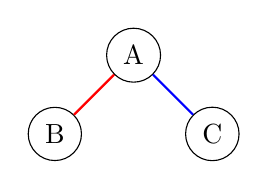
\begin{tikzpicture}

            %\draw [help lines] (0,0) grid (10,10); 

            \path   (5,10)node (a) [circle,draw] {A}
                    (4,9) node (b) [circle,draw] {B}
                    (6,9) node (c) [circle,draw] {C};
                
            \draw[thick,red]  (node cs: name =a ) -- (node cs:name =b);
            \draw[thick,blue] (node cs: name =a ) -- (node cs:name =c);
        \end{tikzpicture}
\end{document}